% Copyright (c) 2010 Milton Mazzarri <milmazz@gmail.com>
% All rights reserved.
% 
% Redistribution and use in source and binary forms, with or without
% modification, are permitted provided that the following conditions
% are met:
% 1. Redistributions of source code must retain the above copyright
%    notice, this list of conditions and the following disclaimer.
% 2. Redistributions in binary form must reproduce the above copyright
%    notice, this list of conditions and the following disclaimer in the
%    documentation and/or other materials provided with the distribution.
% 3. The name of the author may not be used to endorse or promote products
%    derived from this software without specific prior written permission.
% 
% THIS SOFTWARE IS PROVIDED BY THE AUTHOR ``AS IS'' AND ANY EXPRESS OR
% IMPLIED WARRANTIES, INCLUDING, BUT NOT LIMITED TO, THE IMPLIED WARRANTIES
% OF MERCHANTABILITY AND FITNESS FOR A PARTICULAR PURPOSE ARE DISCLAIMED.
% IN NO EVENT SHALL THE AUTHOR BE LIABLE FOR ANY DIRECT, INDIRECT,
% INCIDENTAL, SPECIAL, EXEMPLARY, OR CONSEQUENTIAL DAMAGES (INCLUDING, BUT
% NOT LIMITED TO, PROCUREMENT OF SUBSTITUTE GOODS OR SERVICES; LOSS OF USE,
% DATA, OR PROFITS; OR BUSINESS INTERRUPTION) HOWEVER CAUSED AND ON ANY
% THEORY OF LIABILITY, WHETHER IN CONTRACT, STRICT LIABILITY, OR TORT
% (INCLUDING NEGLIGENCE OR OTHERWISE) ARISING IN ANY WAY OUT OF THE USE OF
% THIS SOFTWARE, EVEN IF ADVISED OF THE POSSIBILITY OF SUCH DAMAGE.

\documentclass{beamer}

% Uso de estilos en beamer
%\usetheme{Frankfurt}
\usetheme{JuanLesPins}
 %AnnArbor
 %Antibes
 %Berlin
 %Boadilla
 %Copenhagen
 %Darmstadt
 %default
 %Dresden
 %Frankfurt
 %Hannover
 %Ilmenau
 %JuanLesPins
 %Madrid
 %Rochester
 %Warsaw
 %}
\useoutertheme{}
\useinnertheme{}
\usefonttheme{}
\usecolortheme{}
%beaver
%beetle
%crane
%default
%dolphin
%dove
%fly
%seagull
%sidebartab

% Desactivar la barra de navegacion
%\setbeamertemplate{navigation symbols}{}

\usepackage[spanish]{babel}
\usepackage[utf8]{inputenc}

% Redefinicion de teorema, definicion, ejemplo
\newtheorem{teorema}[theorem]{Teorema}
\newtheorem{definicion}[theorem]{Definición}
\newenvironment{ejemplo}{\begin{exampleblock}{Ejemplo}}{\end{exampleblock}}

\title{Herramientas libres para el apoyo en el proceso de desarrollo de software}
\subtitle{Trac}
\author[Milton Mazzarri]{Milton Mazzarri \\
\href{mailto:milmazz@gmail.com}{milmazz@gmail.com} \\
}
\institute[gUsLA]{Grupo de Usuarios de Software Libre de la Universidad de Los Andes}
\date{Noviembre, 2007}

\hypersetup{colorlinks=true,linkcolor=blue}

\hypersetup{
pdfauthor={Milton R. Mazzarri S.},
pdftitle={Trac: Manejo y Gestión de Proyectos}
}

 \AtBeginSubsection[]
{
  \begin{frame}<beamer>[allowframebreaks]{Contenido}
    \tableofcontents[currentsection,currentsubsection]
  \end{frame}
}

% Presentacion paso a paso
\beamerdefaultoverlayspecification{<+->}

\begin{document}

\begin{frame}
\titlepage
\end{frame}

\begin{frame}[allowframebreaks]{Contenido}
    \tableofcontents[pausesections]
\end{frame}

\section{Gestión y Seguimiento de Proyectos}
\subsection{Conceptos}
\frame{
    \frametitle{¿Qué es exactamente?}
    
    \begin{itemize}
        \item
            Es un sistema wiki, seguimiento y manejo de proyectos mejorado para el desarrollo de proyectos de software.
        \item
            Uso de un enfoque minimalista para el manejo de proyectos de desarrollo de software basado en la Web.
        \item
            Tiene como misión ayudar a los desarrolladores a escribir software de excelente calidad, mientras busca no interferir en el proceso y políticas del desarrollo.
        \item
            Es multiplataforma.
    \end{itemize}
}

\frame{
    \frametitle{Manejo de Proyectos de Desarrollo de Software}

    \begin{itemize}
        \item
            Herramientas comunes para el manejo de proyectos de software:
                \begin{itemize}
                    \item
                        Sistemas de Seguimiento.
                    \item
                        Sistemas de Control de Versiones.
                    \item
                        Sistemas Wiki.
                \end{itemize}
        \item
            \alert{Problema:} La información del Proyecto no se concentra en un solo lugar.
    \end{itemize}
}

\section{Trac}
\subsection{Propósito}
\frame{
    \frametitle{Propósito}

    \begin{itemize}
        \item
            Ofrecer una interfaz integrada y consistente para acceder a la información del Proyecto:
                \begin{itemize}
                    \item
                        Sistema de seguimiento de errores integrado.
                    \item
                        Sistema Wiki integrado.
                    \item
                        Integración con Sistemas de Control de Versiones.
                    \item
                        Reportes de tickets.
                \end{itemize}
        \item
            Ofrecer un sistema totalmente extensible por medio de plugins.
    \end{itemize}

}

\subsection{Características}

\begin{frame}[fragile]
    \frametitle{Línea de Tiempo}

    \begin{itemize}
        \item
            Registro de eventos ocurridos a diario.
        \item
            Acceso a los registros desde un solo lugar.
        \item
            Ofrecer feeds \alert{RSS}.
    \end{itemize}
    
    \begin{figure}
        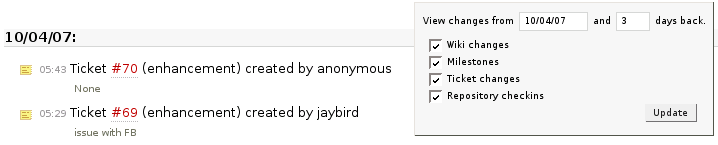
\includegraphics[scale=0.3]{pix/timeline}
        \caption{Línea de tiempo}
    \end{figure}
\end{frame}

\begin{frame}
    \frametitle{Wiki}

    \begin{itemize}
        \item
            Ideal para mantener la base de conocimiento del Proyecto.
        \item
            Mantenimiento de la documentación del Proyecto.
    \end{itemize}

    \begin{figure}
        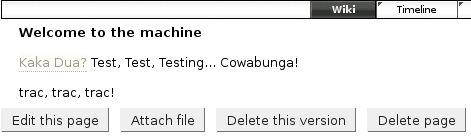
\includegraphics[scale=0.3]{pix/wiki}
        \caption{Sistema Wiki}
    \end{figure}

\end{frame}

\frame{
    \frametitle{Consistencia}

    La misma sintaxis del Wiki es usada en Trac para:
    
    \begin{itemize}
        \item
            Paginas Wiki.
        \item
            Tickets (\emph{bugs}, \emph{issues}).
        \item
            En los mensajes de envío del Sistema de Control de Versiones (\emph{commits})
        \item
            En la descripción de los hitos.
    \end{itemize}
}

\begin{frame}
    \frametitle{Roadmap}

    Muestra el porcentaje de avance de la versión actual del proyecto respecto al número de \emph{tickets activos} vs. \emph{tickets cerrados}.
    
    \begin{figure}
        
\includegraphics[scale=0.3]{pix/roadmap}
        \caption{Vista Roadmap}
    \end{figure}
\end{frame}

\begin{frame}
    \frametitle{Integración con Subversion}

    \begin{columns}

    \begin{column}{5cm}
        \begin{itemize}
            \item<1->
                Visor del código fuente del proyecto.
            \item<3->
                Visualización de diferencias en las revisiones, ficheros, etc.
            \item<6->
                Resaltado de código.
        \end{itemize}
    \end{column}

    \begin{column}{5cm}
        \begin{overprint}
            \includegraphics<2>[scale=0.2]{pix/subversion}
            \includegraphics<4>[scale=0.2]{pix/changeset}
            \includegraphics<5>[scale=0.4]{pix/changeset2}
        \end{overprint}
    \end{column}

    \end{columns}
\end{frame}

\begin{frame}
    \frametitle{Consultas de tickets}

    \begin{figure}
        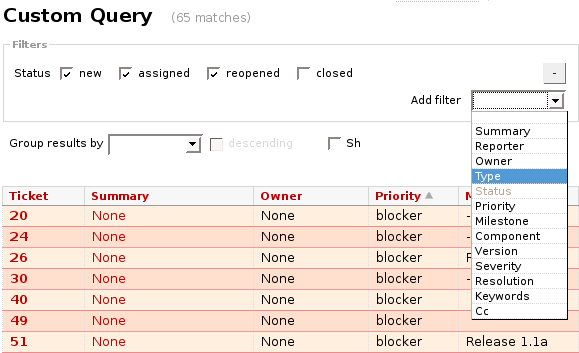
\includegraphics[scale=0.3]{pix/tickets}
        \caption{Consultas de tickets personalizadas}
    \end{figure}

\end{frame}

\begin{frame}[fragile]
    \frametitle{En la unión está la fuerza}

    \begin{ejemplo}
        \begin{verbatim}
            Wiki: CamelCase
            Tickets: #123
            Revisiones: r123
            Codigo: source:trunk/main.cpp
        \end{verbatim}
    \end{ejemplo}
\end{frame}

\subsection{Personalización}

\frame{
    \frametitle{¿Puedo hacer ajustes?}

    \begin{itemize}
        \item
            Cada organización tiene distintas necesidades.
        \item
            Capacidad de escribir extensiones en Python para:
            \begin{description}
                \item[Macros] Definir funciones para usar en el Wiki.
                \item[Plugins] Extender los componentes actuales o agregar nuevos.
            \end{description}
        \item
            Cantidad inmensa de \alert{Macros} y \alert{Plugins} disponibles en diversos proyectos de la comunidad del \emph{Software Libre}.
    \end{itemize}
}

\frame{
    \frametitle{Plugins}

    \begin{itemize}
        \item
            Administración.
        \item
            Control de SPAM.
        \item
            Manejo de cuentas.
        \item
            Compatibilidad con Sistemas de Control.
        \item
            Integración con LDAP.
        \item
            Integración continúa.
        \item
            \ldots
    \end{itemize}
}

\begin{frame}
    \frametitle{Plugin: Bitten}

    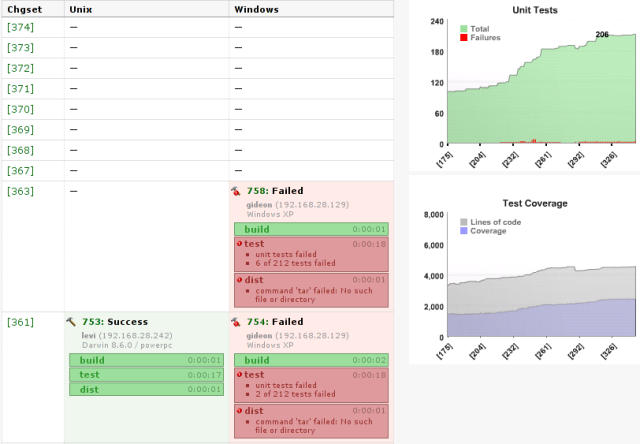
\includegraphics[scale=0.3]{pix/bitten}

\end{frame}

%\begin{frame}
%    \frametitle{¿Quien lo usa?}
%\end{frame}

\section{Referencias}

\frame{
    \frametitle{Enlaces de interés}

    \begin{itemize}
        \item \url{http://trac.edgewall.org/}
        \item \url{http://bitten.edgewall.org/}
        \item \url{http://trac-hacks.org/}
    \end{itemize}
}

\frame{
    \frametitle{¿Preguntas?}

    \begin{itemize}
        \item
            Milton R. Mazzarri S.
        \item
            \href{mailto:milmazz@gmail.com}{milmazz@gmail.com}
        \item
            \href{http://www.milmazz.com.ve}{http://www.milmazz.com.ve}
    \end{itemize}
}

\end{document}
